\documentclass[11pt,a4paper]{article}
\usepackage[margin=18mm,top=22mm,bottom=20mm]{geometry}
\usepackage{fontspec}\setmainfont{Latin Modern Roman}
\usepackage{amsmath,amssymb,tikz,graphicx,fancyhdr,array,needspace}
\setlength{\headheight}{14pt}
\usetikzlibrary{arrows.meta}
\pagestyle{fancy}\fancyhf{}\renewcommand{\headrulewidth}{0.4pt}
\fancyhead[L]{\textbf{M-02}}\fancyhead[C]{\itshape Fizika (OliyFizika.uz mock test)}\fancyhead[R]{\textbf{Mock №2}}
\fancyfoot[C]{\thepage}
\setlength{\parindent}{0pt}\setlength{\parskip}{3pt}
\newcommand{\opt}[2]{\hspace*{4mm}#1)\ #2\par}
\newcommand{\blank}{\rule{5cm}{0.4pt}}
\begin{document}

\begin{center}{\Large\textbf{FIZIKA}}\end{center}
\noindent\begin{minipage}{\linewidth}
\textbf{1.}\ Elastiklik moduli $E$ ga teng bölgan moddadan tayyorlangan, uzunligi $l$, köndalang kesim yuzasi $S$ bölgan elastik arqon berilgan. Uning bir uçiga $m$ massali jism osib vertikal tebratildi. Jismning vertikal tebranişlari davri aniqlansin.\par\smallskip
\opt{A}{$\dfrac{1}{2\pi}\sqrt{\dfrac{ES}{ml}}$}
\opt{B}{$\dfrac{1}{2\pi}\sqrt{\dfrac{ml}{ES}}$}
\opt{C}{$2\pi\sqrt{\dfrac{ES}{ml}}$}
\opt{D}{$2\pi\sqrt{\dfrac{ml}{ES}}$}
\end{minipage}\vspace{9pt}\par
\noindent\begin{minipage}{\linewidth}
\textbf{2.}\ 4 cm ipga osilgan şarça rasmdagi mexanizmda O öq atrofida $\omega$ = 2 rad/s burçak tezlikda aylantirilmoqda. Agar mazkur holatda ip vertikaldan 30$^\circ$ burçakka oğib aylanayotgan bölsa, şarçaning çiziqli tezligini toping (cm/s).\par\smallskip
\noindent\hspace*{4mm}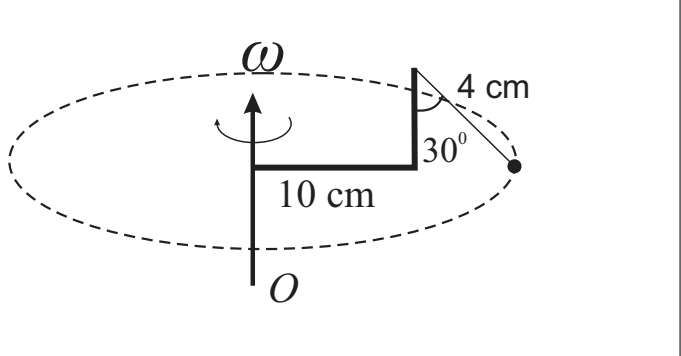
\includegraphics[width=0.6\linewidth,height=5.2cm,keepaspectratio]{../dtm-variantlari/rasmlar/T05-04.png}\par\smallskip
\opt{A}{12}
\opt{B}{2,4}
\opt{C}{24}
\opt{D}{4}
\end{minipage}\vspace{9pt}\par
\noindent\begin{minipage}{\linewidth}
\textbf{3.}\ Blokni kötarib turgan ipning taranglik kuçi 36 N bölsa, blokka ilingan yukning oğirligi (N) aniqlansin. (blok vaznini inobatga olmang)\par\smallskip
\noindent\hspace*{4mm}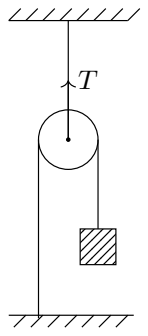
\includegraphics[width=0.6\linewidth,height=5.2cm,keepaspectratio]{../dtm-variantlari/rasmlar/8000897-11.png}\par\smallskip
\opt{A}{36}
\opt{B}{72}
\opt{C}{9}
\opt{D}{18}
\end{minipage}\vspace{9pt}\par
\noindent\begin{minipage}{\linewidth}
\textbf{4.}\ Jismga 69 N va 74 N kuçlar qöyilgan. Bu kuçlarning natijavyisi 5 N bölsa, ular orasidagi burçakni aniqlang.\par\smallskip
\opt{A}{90$^\circ$}
\opt{B}{150$^\circ$}
\opt{C}{180$^\circ$}
\opt{D}{60$^\circ$}
\end{minipage}\vspace{9pt}\par
\noindent\begin{minipage}{\linewidth}
\textbf{5.}\ Şişa nayning uçi yengil plastinka bilan berkitilib, suvga 0,34 m çuqurlikka botirilgan. Nayga qança qalinlikda (m) simob ($\rho$=13600 kg/m$^{3}$) quyilsa, plastinka tuşib ketadi?\par\smallskip
\opt{A}{0,25}
\opt{B}{0,05}
\opt{C}{0,025}
\opt{D}{0,005}
\end{minipage}\vspace{9pt}\par
\noindent\begin{minipage}{\linewidth}
\textbf{6.}\ Mix ombur bilan qisildi. Omburning aylaniş öqidan mixgaça bölgan masofa 2 cm, qöl kuçi qöyilgan nuqtagaça esa 16 cm. Qöl omburni 200 N kuç bilan qisadi. Mixga ta’sir qiluvçi kuçni toping (N).\par\smallskip
\opt{A}{16}
\opt{B}{160}
\opt{C}{1600}
\opt{D}{16000}
\end{minipage}\vspace{9pt}\par
\noindent\begin{minipage}{\linewidth}
\textbf{7.}\ Nima uçun zilzila payti odam yer qimirlaşini 2 marta sezadi?\par\smallskip
\opt{A}{çunki, zil zila markazidan odamga böylama tölqin birinçi bölib yetib keladi}
\opt{B}{çunki, zil zila markazidan odamga köndalang tölqin birinçi bölib yetib keladi}
\opt{C}{çunki, zil zila markazidan odamga böylama va köndalang tölqin bir vaqtda yetib keladi}
\opt{D}{bunday hodisa kuzatilmaydi}
\end{minipage}\vspace{9pt}\par
\noindent\begin{minipage}{\linewidth}
\textbf{8.}\ Kosmik kema vertikal yönalişda (Oyga nisbatan) 8,38 m/s$^{2}$ özgarmas tezlaniş bilan sekinlanuvçan harakatlanib, Oyga yumşoq qönadi. Şu kemadagi massasi 70 kg bölgan kosmonavtning oğirligi qança böladi (N)? g=1,62 N/kg.\par\smallskip
\opt{A}{700}
\opt{B}{800}
\opt{C}{600}
\opt{D}{300}
\end{minipage}\vspace{9pt}\par
\noindent\begin{minipage}{\linewidth}
\textbf{9.}\ Jism OX öqida v = 10+4t [m/s] qonuniyat böyiça harakatlanmoqda. Uning tezlanişi qançaga (m/s$^{2}$) teng?\par\smallskip
\opt{A}{2}
\opt{B}{4}
\opt{C}{1}
\opt{D}{10}
\end{minipage}\vspace{9pt}\par
\noindent\begin{minipage}{\linewidth}
\textbf{10.}\ Gorizontal tekislikda arqon yordamida 11 kg massali çana tekis tortib ketilmoqda. Agar arqon gorizont bilan taşkil qilgan burçagining tangensi 0,75 ga teng bölsa, arqonning taranglik kuçini toping (N). Işqalaniş koeffitsiyenti 0,5 ga teng. g=10 N/kg.\par\smallskip
\opt{A}{30}
\opt{B}{20}
\opt{C}{50}
\opt{D}{15}
\end{minipage}\vspace{9pt}\par
\noindent\begin{minipage}{\linewidth}
\textbf{11.}\ Yoy şaklida bukilgan yengil plastina kuçli qizdirilib issiqlikdan juda tez kengayuvçi taglikka qöyildi. Mazkur holatda plastina özini qanday tutadi? Taglikda issiqlikdan kengayiş faqat plastina tegib turgan sohada yuz beradi.\par\smallskip
\noindent\hspace*{4mm}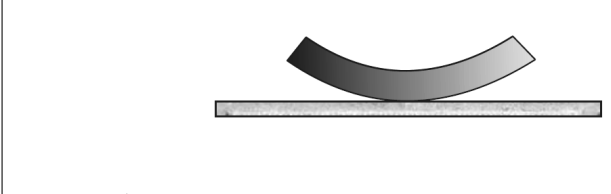
\includegraphics[width=0.6\linewidth,height=5.2cm,keepaspectratio]{../dtm-variantlari/rasmlar/T12-15.png}\par\smallskip
\opt{A}{plastina bir tarafga qiyalab qoladi}
\opt{B}{plastina tinç turadi}
\opt{C}{plastina tinç turadi yoki tebranma harakatga keladi}
\opt{D}{plastina tinç turadi yoki bir tarafga qiyalab qoladi}
\end{minipage}\vspace{9pt}\par
\noindent\begin{minipage}{\linewidth}
\textbf{12.}\ FIK 50 \% bölgan elektroplita yordamida 132 g qaynagan suvni neça minutda buğlantiriş mumkin? Tok kuçi 4,6 A, kuçlaniş 220 V hamda suvning buğ hosil qiliş issiqligi 2,3 MJ/kg.\par\smallskip
\opt{A}{600}
\opt{B}{101}
\opt{C}{9}
\opt{D}{10}
\end{minipage}\vspace{9pt}\par
\noindent\begin{minipage}{\linewidth}
\textbf{13.}\ Ideal gaz birinçi holatdan ikkinçi holatga ötganda temperaturasi 350 $^\circ$C ga özgardi. Agar $p_1$=58 kPa, $p_2$=29 kPa bölsa, gazning dastlabki temperaturasi (K) qanday bölgan?\par\smallskip
\noindent\hspace*{4mm}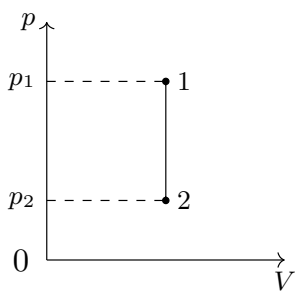
\includegraphics[width=0.6\linewidth,height=5.2cm,keepaspectratio]{../dtm-variantlari/rasmlar/8000273-02.png}\par\smallskip
\opt{A}{650}
\opt{B}{350}
\opt{C}{700}
\opt{D}{300}
\end{minipage}\vspace{9pt}\par
\noindent\begin{minipage}{\linewidth}
\textbf{14.}\ $m$ massali ideal gaz ustida grafikda körsatilganidek I va II jarayonlar amalga oşirildi. Agar $B$ va $A$ nuqtalarga mos keluvchi bosimlar nisbati $p_B/p_A$=3 bölsa, bu nuqtalarga mos keluvchi hajmlar nisbati $V_B/V_A$ ni aniqlang.\par\smallskip
\noindent\hspace*{4mm}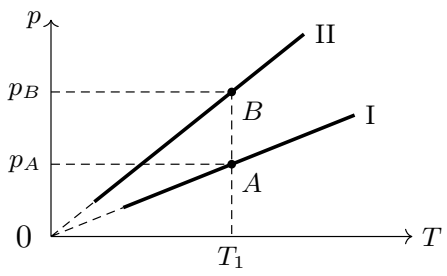
\includegraphics[width=0.6\linewidth,height=5.2cm,keepaspectratio]{../dtm-variantlari/rasmlar/8000297-19.png}\par\smallskip
\opt{A}{1/9}
\opt{B}{9}
\opt{C}{3}
\opt{D}{1/3}
\end{minipage}\vspace{9pt}\par
\noindent\begin{minipage}{\linewidth}
\textbf{15.}\ Karno siklida işlayotgan sovutiş rejimidagi issiqlik maşinasi uçun Karno sikli qaysi yönalişda amalga oşadi? Bir siklda işçi jismning içki energiyasi qanday özgaradi?\par\smallskip
\opt{A}{soat miliga teskari yönalişda; ortadi}
\opt{B}{soat mili yönalişda; özgarmaydi}
\opt{C}{soat miliga teskari yönalişda; özgarmaydi}
\opt{D}{soat mili yönalişda; kamayadi}
\end{minipage}\vspace{9pt}\par
\noindent\begin{minipage}{\linewidth}
\textbf{16.}\ Nuqtaviy zaryad atrofidagi ikki nuqtada elektr maydon kuçlanganliklari 81 marta farq qiladi. Bu nuqtalardan zaryadgaça bölgan masofalar nisbati qanday?\par\smallskip
\opt{A}{2}
\opt{B}{27}
\opt{C}{9}
\opt{D}{3}
\end{minipage}\vspace{9pt}\par
\noindent\begin{minipage}{\linewidth}
\textbf{17.}\ Maydon kuçlanganligi 200 kV/m bölgan bir jinsli elektr maydonida elektronga ta’sir etuvçi kuçni aniqlang (N).\par\smallskip
\opt{A}{3,2 $\cdot$ 10$^{-14}$}
\opt{B}{1,6 $\cdot$ 10$^{-14}$}
\opt{C}{3,2 $\cdot$ 10$^{-11}$}
\opt{D}{1,6 $\cdot$ 10$^{-11}$}
\end{minipage}\vspace{9pt}\par
\noindent\begin{minipage}{\linewidth}
\textbf{18.}\ Tomoni $a$ bölgan teng tomonli uçburçakning uçlarida $q$, $2q$, $3q$ zaryadli nuqtaviy zarralar joylaşgan. Zaryadi $q$, massasi $m$ bölgan zarra böşatib yuborilsa, u qanday maksimal tezlikka erişadi?\par\smallskip
\opt{A}{$\sqrt{\dfrac{18kq^2}{ma}}$}
\opt{B}{$\sqrt{\dfrac{6kq}{ma}}$}
\opt{C}{$\sqrt{\dfrac{18kq}{ma}}$}
\opt{D}{$\sqrt{\dfrac{10kq^2}{ma}}$}
\end{minipage}\vspace{9pt}\par
\noindent\begin{minipage}{\linewidth}
\textbf{19.}\ Massalari $m$ dan bölgan $q$ va $3q$ zaryadli zarralar bir biridan $a$ masofada uşlab turilibdi. $q$ zaryadli zarra böşatib yuborilsa, u qanday maksimal tezlikka erişadi?\par\smallskip
\opt{A}{$\sqrt{\dfrac{3q^2}{am}}$}
\opt{B}{$\sqrt{\dfrac{6kq^2}{am}}$}
\opt{C}{$\sqrt{\dfrac{12kq}{am}}$}
\opt{D}{$\sqrt{\dfrac{18kq}{am}}$}
\end{minipage}\vspace{9pt}\par
\noindent\begin{minipage}{\linewidth}
\textbf{20.}\ Tölqin uzunligi qanday bölgan nurlar bilan yoritilayotgan katoddan uçib çiqayotgan fotoelektronlarni batamom tormozlaş uçun katod va anod orasidagi potensiallar ayirmasi 0,75 V ga teng böladi? Çiqiş işi 3 eV ga teng.\par\smallskip
\opt{A}{331 nm}
\opt{B}{640 $\mu$m}
\opt{C}{331 pm}
\opt{D}{400 nm}
\end{minipage}\vspace{9pt}\par
\noindent\begin{minipage}{\linewidth}
\textbf{21.}\ $R$ radiusli $q$ zaryadga ega şar sirtidan $R$ masofadagi nuqtada maydon potensiali $\varphi$ edi. Bu şarga qöşimça zaryad berildi. Natijada şar sirtidan 3$R$ masofadagi maydon potensiali ham $\varphi$ ni taşkil etdi. Qöşimça berilgan zaryad midorini aniqlang.\par\smallskip
\opt{A}{4$q$}
\opt{B}{$q$}
\opt{C}{2$q$}
\opt{D}{3$q$}
\end{minipage}\vspace{9pt}\par
\noindent\begin{minipage}{\linewidth}
\textbf{22.}\ Misdan ikki silindrsimon ötkazgiçlar tayyorlangan. Ikkinçisining köndalang kesim radiusi 2 marta katta, ammo uzunligi 4 marta kiçik. Ularning qarşiliklarining nisbati $R_1/R_2$ ni toping.\par\smallskip
\opt{A}{1/16}
\opt{B}{1/8}
\opt{C}{8}
\opt{D}{16}
\end{minipage}\vspace{9pt}\par
\noindent\begin{minipage}{\linewidth}
\textbf{23.}\ Effektiv qiymati 2 A bölgan özgaruvçan tok aktiv qarşiligi 1,5 $\Omega$ bölgan elektr zanjir uçlarida 4 V effektiv kuçlaniş hosil qilinmoqda. Zanjirning quvvat koeffitsiyentini toping.\par\smallskip
\opt{A}{0,5}
\opt{B}{0,75}
\opt{C}{0,6}
\opt{D}{0,45}
\end{minipage}\vspace{9pt}\par
\noindent\begin{minipage}{\linewidth}
\textbf{24.}\ Töyiniş toki 80 mA bölsa, katod sirtidan har sekundda neçta elektron uçib çiqadi? e=1,6$\cdot10^{-19}$ C.\par\smallskip
\opt{A}{5$\cdot10^{17}$}
\opt{B}{2$\cdot10^{15}$}
\opt{C}{2$\cdot10^{16}$}
\opt{D}{2$\cdot10^{14}$}
\end{minipage}\vspace{9pt}\par
\noindent\begin{minipage}{\linewidth}
\textbf{25.}\ Elektr maydonda 1 $\mu$g massali çang zarrasi vertikal ravişda 4 sekundda yerga tuşdi. Agar maydon kuçlanganligi 50 V/m va maydon kuç çiziqlari tik yuqoriga yönalgan bölsa, çang zarrasi qanday balandlikdan tuşgan (m)? Çang zarrasi zaryadi 0,02 nC.\par\smallskip
\opt{A}{80}
\opt{B}{63}
\opt{C}{79}
\opt{D}{72}
\end{minipage}\vspace{9pt}\par
\noindent\begin{minipage}{\linewidth}
\textbf{26.}\ Lupa orqali qaragan momentda unda 11 ga teng optimal (körinma) kattalaştiriş yuzaga keladi. Birozdan keyin köz çarçaşi oqibatida akkomodatsiyalanadi. Natijada lupaning kattalaştirişi nimaga teng bölib qoladi?\par\smallskip
\opt{A}{10}
\opt{B}{11}
\opt{C}{5,5}
\opt{D}{8}
\end{minipage}\vspace{9pt}\par
\noindent\begin{minipage}{\linewidth}
\textbf{27.}\ Botiq közguning egrilik radiusi 24 cm. Uning fokus masofasini (cm) aniqlang.\par\smallskip
\opt{A}{24}
\opt{B}{6}
\opt{C}{12}
\opt{D}{48}
\end{minipage}\vspace{9pt}\par
\noindent\begin{minipage}{\linewidth}
\textbf{28.}\ Optik kuçi 2 D bölgan yiğuvçi linzadan ikkilangan fokus masofada turgan buyum 1 m/s tezlik bilan linza tomon harakatlana boşladi. Bundan 0,75 s vaqt ötgan paytda buyum va uning tasviri orasidagi masofa qanday böladi (m)?\par\smallskip
\opt{A}{0,5}
\opt{B}{0,25}
\opt{C}{0,75}
\opt{D}{0,15}
\end{minipage}\vspace{9pt}\par
\noindent\begin{minipage}{\linewidth}
\textbf{29.}\ Yoruğlik tezligiga yaqin tezlik bilan harakatlanayotgan jismning massasi tinçlikdagi massasiga nisbatan 4 marta ortdi. Uning uzunligi qanday özgarganini aniqlang.\par\smallskip
\opt{A}{2 marta ortgan}
\opt{B}{2 marta kamaygan}
\opt{C}{4 marta kamaygan}
\opt{D}{4 marta ortgan}
\end{minipage}\vspace{9pt}\par
\noindent\begin{minipage}{\linewidth}
\textbf{30.}\ Radioaktiv yemiriliş natijasida uran 238 92 U 206 qörğoşinga 82 P aylandi. Neçta $\alpha$ va $\beta$ yemirilişlar yuz bergan?\par\smallskip
\opt{A}{8$\alpha$ va 6$\beta$}
\opt{B}{4$\alpha$ va 6$\beta$}
\opt{C}{6$\alpha$ va 8$\beta$}
\opt{D}{5$\alpha$ va 8$\beta$}
\end{minipage}\vspace{9pt}\par
\noindent\begin{minipage}{\linewidth}
\textbf{31.}\ Harorati 27 $^\circ$C bölgan 2 mol bir atomli ideal gazning ilgarilanma harakatidagi töliq kinetik energiyasini aniqlang. Universal gaz doimiysi 8,31 J/(mol$\cdot$K).\par\smallskip
\opt{A}{1007}
\opt{B}{7964}
\opt{C}{6540}
\opt{D}{7479}
\end{minipage}\vspace{9pt}\par
\noindent\begin{minipage}{\linewidth}
\textbf{32.}\ 5 cm ga siqilgan prujinaning potensial energiyasi 10 J. Prujinaning bikrligini (kN/m) aniqlang.\par\smallskip
\opt{A}{8}
\opt{B}{12}
\opt{C}{4}
\opt{D}{16}
\end{minipage}\vspace{9pt}\par
\newpage\noindent\textbf{33–35-test topshiriqlariga mos keluvchi javoblarni (A–F) javob variantlaridan tanlang.}\par\smallskip
Rasmda elektr zanjir tasvirlangan. Batareyaning ichki qarshiligi nolga teng, ampermetrlar ideal.\par\medskip
\begin{center}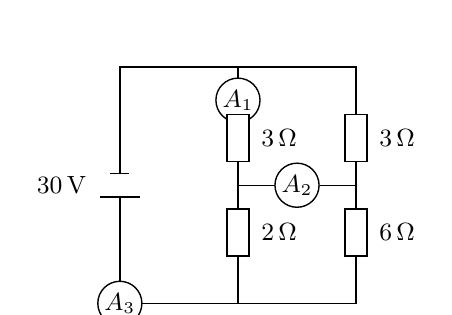
\begin{tikzpicture}[line width=0.5pt]
\draw (0,0)--(0,1.35); \draw (0,1.65)--(0,3)--(3,3)--(3,2.4); \draw (-0.25,1.35)--(0.25,1.35); \draw (-0.12,1.65)--(0.12,1.65);
\node[left] at (-0.3,1.5) {\small $30\,\mathrm{V}$};
\draw (1.5,3)--(1.5,2.72); \draw (1.5,2.44)--(1.5,2.4);
\draw (1.5,1.8)--(1.5,1.2); \draw (1.5,0.6)--(1.5,0)--(0.28,0); \draw (-0.28,0)--(0,0);
\draw (3,1.8)--(3,1.2); \draw (3,0.6)--(3,0)--(1.5,0);
\draw (1.5,1.5)--(1.97,1.5); \draw (2.53,1.5)--(3,1.5);
\draw[fill=white] (1.5,2.58) circle (0.28); \node at (1.5,2.58) {\small $A_1$};
\draw[fill=white] (1.3599999999999999,1.8) rectangle (1.6400000000000001,2.4); \node[right] at (1.67,2.1) {\small $3\,\Omega$};
\draw[fill=white] (1.3599999999999999,0.6000000000000001) rectangle (1.6400000000000001,1.2); \node[right] at (1.67,0.9) {\small $2\,\Omega$};
\draw[fill=white] (2.86,1.8) rectangle (3.14,2.4); \node[right] at (3.17,2.1) {\small $3\,\Omega$};
\draw[fill=white] (2.86,0.6000000000000001) rectangle (3.14,1.2); \node[right] at (3.17,0.9) {\small $6\,\Omega$};
\draw[fill=white] (2.25,1.5) circle (0.28); \node at (2.25,1.5) {\small $A_2$};
\draw[fill=white] (0.0,0.0) circle (0.28); \node at (0.0,0.0) {\small $A_3$};
\end{tikzpicture}\end{center}
\noindent\fbox{\begin{minipage}{0.64\linewidth}\vspace{4pt}\textbf{33.}\ $A_1$ ampermetrning körsatişini (A) aniqlang.\\[6pt]\textbf{34.}\ $A_2$ ampermetrning körsatişini (A) aniqlang.\\[6pt]\textbf{35.}\ $A_3$ ampermetrning körsatişini (A) aniqlang.\vspace{4pt}\end{minipage}\vrule\hspace{6pt}\begin{minipage}{0.28\linewidth}\vspace{4pt}A)\ 5\\B)\ 7,5\\C)\ 12,5\\D)\ 2,5\\E)\ 10\\F)\ 3,5\vspace{4pt}\end{minipage}}\par\vspace{14pt}
\Needspace{9\baselineskip}
\noindent\textbf{36.}\ Qirrasining uzunligi 3 cm bölgan kub şaklidagi 2 ta muz bölagi asosining yuzasi 100 cm$^2$ bölgan, 101,4 g suv quyilgan silindrik idişda taşlandi. $\rho_{muz}=900$ kg/m$^3$.\par\smallskip
\medskip\noindent\textbf{a)\ Muzlar erib ketgandan söng suyuqlikning idiş tubiga beradigan bosimini (Pa) toping.}\par
\noindent\textit{Javob}: a)\ \blank\par
\medskip\noindent\textbf{b)\ Muzlar erib ketgandan söng suyuqlikning idiş tubiga beradigan bosim kuçini (N) hisoblang.}\par
\noindent\textit{Javob}: b)\ \blank\par
\medskip\noindent\textbf{Diqqat!} Javoblaringizni javoblar varaqasiga köçirib yozing.\par\vspace{10pt}
\Needspace{9\baselineskip}
\noindent\textbf{37.}\ Silindrik idişga teng massali suv va kerosin quyildi. Suyuqliklar ustunining umumiy balandligi 18 cm ga teng. $\rho_{kerosin}=800$ kg/m$^3$.\par\smallskip
\medskip\noindent\textbf{a)\ Suv ustunining balandligini (cm) aniqlang.}\par
\noindent\textit{Javob}: a)\ \blank\par
\medskip\noindent\textbf{b)\ Idiş tubidan 4 cm balandlikdagi nuqtada suyuqliklarning hosil qilgan umumiy bosimini (Pa) toping.}\par
\noindent\textit{Javob}: b)\ \blank\par
\medskip\noindent\textbf{Diqqat!} Javoblaringizni javoblar varaqasiga köçirib yozing.\par\vspace{10pt}
\Needspace{9\baselineskip}
\noindent\textbf{38.}\ Uzunligi 4 m, qiyalik burçagi $53^\circ$ bölgan silliq qiya tekislik tepasidan 10 kg massali jism sirpanib tuşdi. $\sin53^\circ=0,8$, $\cos53^\circ=0,6$.\par\smallskip
\medskip\noindent\textbf{a)\ Jismning qiya tekislik etagidagi tezligini (m/s) toping.}\par
\noindent\textit{Javob}: a)\ \blank\par
\medskip\noindent\textbf{b)\ Bu jarayonda oğirlik kuçining bajargan işini (J) toping.}\par
\noindent\textit{Javob}: b)\ \blank\par
\medskip\noindent\textbf{Diqqat!} Javoblaringizni javoblar varaqasiga köçirib yozing.\par\vspace{10pt}
\Needspace{9\baselineskip}
\noindent\textbf{39.}\ Bir atomli ideal gazga 100 J issiqlik berib, hajmi izobarik ravişda 2 marta oşirildi.\par\smallskip
\medskip\noindent\textbf{a)\ Bunda gazning absolyut temperaturasi qanday özgaradi?}\par
\noindent\textit{Javob}: a)\ \blank\par
\medskip\noindent\textbf{b)\ Gazning bajargan işini (J) aniqlang.}\par
\noindent\textit{Javob}: b)\ \blank\par
\medskip\noindent\textbf{Diqqat!} Javoblaringizni javoblar varaqasiga köçirib yozing.\par\vspace{10pt}
\Needspace{9\baselineskip}
\noindent\textbf{40.}\ Issiqlik siğimi 400 J/K bölgan idişda 20 $^\circ$C temperaturali 4 $\ell$ suv bor. Idişga $-10\,^\circ$C temperaturali 1,5 kg muz taşlandi. $c_{suv}=4200$ J/(kg$\cdot$K), $c_{muz}=2100$ J/(kg$\cdot$K), $\lambda_{muz}=330$ kJ/kg.\par\smallskip
\medskip\noindent\textbf{a)\ Natijaviy temperaturani ($^\circ$C) toping.}\par
\noindent\textit{Javob}: a)\ \blank\par
\medskip\noindent\textbf{b)\ Muzning olgan issiqlik miqdorini (kJ) aniqlang.}\par
\noindent\textit{Javob}: b)\ \blank\par
\medskip\noindent\textbf{Diqqat!} Javoblaringizni javoblar varaqasiga köçirib yozing.\par\vspace{10pt}
\Needspace{9\baselineskip}
\noindent\textbf{41.}\ Elektron induksiyasi $B$ bölgan magnit maydonga tik uçib kirdi va $r$ radiusli aylana böylab harakatlana boşladi. $m_e$ — zarraning massasi, $e$ — elementar zaryad.\par\smallskip
\medskip\noindent\textbf{a)\ Uning aylaniş davrini aniqlang.}\par
\noindent\textit{Javob}: a)\ \blank\par
\medskip\noindent\textbf{b)\ Elektronning kinetik energiyasini aniqlang.}\par
\noindent\textit{Javob}: b)\ \blank\par
\medskip\noindent\textbf{Diqqat!} Javoblaringizni javoblar varaqasiga köçirib yozing.\par\vspace{10pt}
\Needspace{9\baselineskip}
\noindent\textbf{42.}\ Maydon kuçlanganligi $E$ bölgan bir jinsli elektr maydonda harakatlanayotgan proton $l$ masofaga köçib, $A$ nuqtadan $B$ nuqtaga yetib bordi (rasmda $AD\perp \vec E$).\par\smallskip
\begin{center}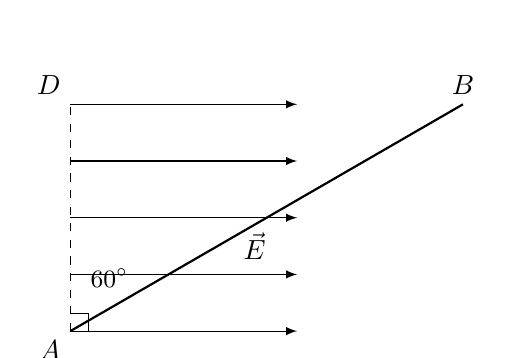
\begin{tikzpicture}[scale=0.9]\foreach \y in {0,0.8,1.6,2.4,3.2}{\draw[-latex] (0,\y)--(3.2,\y);}\draw (0.25,0)--(0.25,0.25)--(0,0.25);\draw[dashed] (0,0)--(0,3.2);\draw[thick] (0,0)--(5.54,3.2);\node[below left] at (0,0) {$A$};\node[above left] at (0,3.2) {$D$};\node[above] at (5.54,3.2) {$B$};\node at (2.6,1.2) {$\vec E$};\node at (0.55,0.75) {\small $60^\circ$};\end{tikzpicture}\end{center}
\medskip\noindent\textbf{a)\ Zarraning kinetik energiyasi qançaga özgarganini aniqlang.}\par
\noindent\textit{Javob}: a)\ \blank\par
\medskip\noindent\textbf{b)\ Zarra $ABDA$ yopiq yöl böylab köçirilganda elektr kuçlar bajaradigan işni aniqlang.}\par
\noindent\textit{Javob}: b)\ \blank\par
\medskip\noindent\textbf{Diqqat!} Javoblaringizni javoblar varaqasiga köçirib yozing.\par\vspace{10pt}
\Needspace{9\baselineskip}
\noindent\textbf{43.}\ Suvdagi nurning intensivligi 45 W/m$^2$ ga teng. $c=3\cdot10^8$ m/s.\par\smallskip
\medskip\noindent\textbf{a)\ Nurdagi elektromagnit maydon energiyasining ziçligini (J/m$^3$) aniqlang.}\par
\noindent\textit{Javob}: a)\ \blank\par
\medskip\noindent\textbf{b)\ Nur suvdagi közgudan tik akslansa, közguga beradigan bosimini (Pa) aniqlang.}\par
\noindent\textit{Javob}: b)\ \blank\par
\medskip\noindent\textbf{Diqqat!} Javoblaringizni javoblar varaqasiga köçirib yozing.\par\vspace{10pt}
\Needspace{9\baselineskip}
\noindent\textbf{44.}\ Quyoşning diametri $13,8\cdot10^{8}$ m ga, Yer bilan Quyoşn orasidagi masofa $1,5\cdot10^{11}$ m ga teng. Fokus masofasi 0,25 m bölgan Yerdagi linza ekranda Quyoşnning haqiqiy tasvirini hosil qilmoqda.\par\smallskip
\medskip\noindent\textbf{a)\ Tasvir bilan linza orasidagi masofani (mm) toping.}\par
\noindent\textit{Javob}: a)\ \blank\par
\medskip\noindent\textbf{b)\ Quyoşn tasvirining diametrini (mm) toping.}\par
\noindent\textit{Javob}: b)\ \blank\par
\medskip\noindent\textbf{Diqqat!} Javoblaringizni javoblar varaqasiga köçirib yozing.\par\vspace{10pt}
\Needspace{9\baselineskip}
\noindent\textbf{45.}\ Ğalayonlangan vodorod atomining ionlaşiş energiyasi 13,6 eV ga teng.\par\smallskip
\medskip\noindent\textbf{a)\ Atom fotonni yutib impuls momentini $2\hbar$ ga oşirsa, uning ionlaniş energiyasi (eV) nimaga teng bölişini aniqlang.}\par
\noindent\textit{Javob}: a)\ \blank\par
\medskip\noindent\textbf{b)\ Atom fotonni yutib impuls momentini $2\hbar$ ga oşirsa, undagi elektronning tezligi neça marta özgarişini aniqlang.}\par
\noindent\textit{Javob}: b)\ \blank\par
\medskip\noindent\textbf{Diqqat!} Javoblaringizni javoblar varaqasiga köçirib yozing.\par\vspace{10pt}
\end{document}